\documentclass[a4paper]{article}

% Packages
\usepackage{amsmath}
\usepackage{amssymb}
\usepackage{amsthm}
\usepackage{bold-extra}
\usepackage{fancyhdr}
\usepackage{geometry}
\usepackage{graphicx}
\usepackage{hyperref}
\usepackage{ifthen}
\usepackage[utf8]{inputenc}
\usepackage{multirow}
\usepackage{needspace}
\usepackage{parskip}
\usepackage{stmaryrd}
\usepackage{listings}
\usepackage[T1]{fontenc}
\usepackage{longtable}
\usepackage{comment}
\usepackage{enumerate}
\usepackage{xspace}
\usepackage{textcomp}
\usepackage{array}

\usepackage{tikz}
\usetikzlibrary{automata,positioning,shapes.geometric}
\usepackage{tikzsymbols}
\usepackage{todonotes}

\lstset{language=Java, numbers=left, showstringspaces=false, tabsize=4}
\geometry{a4paper, left=25mm,right=25mm, top=25mm, bottom=25mm}

% check for the existence of commands
\newcommand{\checkfor}[3]{%
  \ifcsname#1\endcsname%
  #2
  \else%
  #3
  \fi%
}

\checkfor{exnumber}{}{\newcommand{\exnumber}{-1}}

\newcommand{\exercisepagebreak}{\checkfor{isexercise}{\pagebreak}{}}
\newcommand{\solutionpagebreak}{\checkfor{isexercise}{}{\pagebreak}}

\setcounter{section}{\exnumber{}}

\numberwithin{equation}{section}
\numberwithin{figure}{section}
\numberwithin{table}{section}
\renewcommand{\qedsymbol}{\textsc{q.e.d.}}
\renewenvironment{proof}[1][\proofname]{{\bfseries #1: }}{\qed}
\newtheoremstyle{defstyle}{10pt}{5pt}{\addtolength{\leftskip}{2\leftmargini}\addtolength{\rightskip}{2\leftmargini}}{-1\leftmargini}{\scshape\bfseries}{:}{\newline}{#1 #2\ifthenelse {\equal {#3}{}} {}{ (\text{\textsc{#3}})}}{}
\newtheoremstyle{thmstyle}{10pt}{5pt}{\addtolength{\leftskip}{2\leftmargini}\addtolength{\rightskip}{2\leftmargini} \slshape}{-1\leftmargini}{\scshape\bfseries}{:}{\newline}{#1 #2\ifthenelse {\equal {#3}{}} {}{ (\text{\textsc{#3}})}}{}
\newtheoremstyle{exstyle}{10pt}{5pt}{\addtolength{\leftskip}{2\leftmargini}\addtolength{\rightskip}{2\leftmargini}}{-1\leftmargini}{\scshape\bfseries}{:}{\newline}{#1 #2\ifthenelse {\equal {#3}{}} {}{ (\text{\textsc{#3}})}}{}
\newtheoremstyle{algostyle}{10pt}{5pt}{\addtolength{\leftskip}{2\leftmargini}\addtolength{\rightskip}{2\leftmargini}}{-1\leftmargini}{\scshape\bfseries}{:}{\newline}{#1\ifthenelse {\equal {#3}{}} { #2}{ \text{\textsc{#3}}}}{}
\theoremstyle{defstyle}
\newtheorem{mydef}{Definition}[section]
\theoremstyle{thmstyle}
\newtheorem{mythm}{Theorem}[section]
\newtheorem{mylem}[mythm]{Lemma}
\newtheorem{myprop}[mythm]{Proposition}
\theoremstyle{exstyle}
\newtheorem{myex}{Example}[section]
\theoremstyle{algostyle}
\newtheorem{myalgo}{Algorithm}

% Define programming and solution environment and only use if enabled
\checkfor{isprog}{
  % Define exercise environment
  \newcounter{exercise}
  \newenvironment{exercise}[1]{\refstepcounter{exercise}\label{ex\theexercise}\section*{Programming Exercise \theexercise \hfill (#1 Points)}}{}
  \checkfor{isexercise}{
    % Programming exercise
    \excludecomment{solution}
    \excludecomment{onlysolution}
    \newenvironment{onlyexercise}{}{}
    \newcommand{\extitle}{Programming Exercise}
  }{
    % Programming solution
    \newenvironment{solution}{\label{sol\theexercise}\subsection*{Solution: \hrulefill}}{}
    \newenvironment{onlysolution}{}{}
    \excludecomment{onlyexercise}
    \newcommand{\extitle}{Programming Solution}
    }
}{
  % Define exercise environment
  \newcounter{exercise}
  \newenvironment{exercise}[1]{\refstepcounter{exercise}\label{ex\theexercise}\section*{Exercise \theexercise \hfill (#1 Points)}}{}
  \checkfor{isexercise}{
    % Theoretical exercise
    \excludecomment{solution}
    \excludecomment{onlysolution}
    \newenvironment{onlyexercise}{}{}
    \newcommand{\extitle}{Exercise Sheet}
  }{
    % Theoretical solution
    \newenvironment{solution}{\label{sol\theexercise}\subsection*{Solution: \hrulefill}}{}
    \newenvironment{onlysolution}{}{}
    \excludecomment{onlyexercise}
    \newcommand{\extitle}{Solution}
  }
}

% Define header
\pagestyle{fancy}
\fancyhf{} % Clear all headers
\setlength{\headsep}{25pt}
\cfoot{\thepage} % Page numbers
\lhead{ % Header-Definition
  % Logo
  \begin{tabular}[b]{l l}
      \multirow{2}{38mm}{
        \raisebox{-3.6mm}[0pt][0pt]{
          
\includegraphics[height=14mm]{../i2}
        }
      }
      & Lehrstuhl f{\"u}r Informatik 2 \\
      & Software Modeling and Verification
    \end{tabular}
}
\rhead{ % Header-Definition
  % Course name
  \begin{tabular}[b]{r}
    Compiler Construction 2025\\
    \extitle{} \exnumber
  \end{tabular}
}
\AtBeginDocument{
  \vspace*{-30pt}
  apl.\ Prof.\ Dr.\ Thomas Noll\hfill Daniel Zilken, Roy Hermanns
  \vspace{5mm}
}


\newcommand{\header}[1]{
  % Header
  \begin{center}
    {\huge \textbf{Compiler Construction 2025}}\\
    \vspace*{1\baselineskip}%
    {\huge \textbf{--- \extitle{} \exnumber{} ---}}\\
    \checkfor{isexercise}{
      \vspace*{1\baselineskip}
      \checkfor{isprog}{
        %Upload in Moodle until #1 before the exercise class.
      }{
        Upload in Moodle or hand in until #1 before the exercise class.
      }
    }{}
    \vspace*{1.5\baselineskip}
    \hrule
  \end{center}
}

% Change numbering to (a) and (i)
\renewcommand{\labelenumi}{(\alph{enumi})}
\renewcommand{\labelenumii}{(\roman{enumii})}

% Custom commands
\newcommand{\TODO}[1]{\color{red}\textbf{TODO:} #1\color{black}}

% Macros
\newcommand{\set}[1]{\ensuremath{\left\{ #1 \right\}}}
\newcommand{\Nats}{\ensuremath{\mathbb{N}}}
\newcommand{\Reals}{\ensuremath{\mathbb{R}}}

\newcommand{\PTIME}{\mbox{\rm PTIME}}
\newcommand{\PSPACE}{\mbox{\rm PSPACE}}
\newcommand{\coNP}{\mbox{\rm coNP}}
\newcommand{\NP}{\mbox{\rm NP}}
\newcommand{\poly}{\mbox{\rm poly}}
\newcommand{\coPTIME}{\mbox{\rm coPTIME}}
\newcommand{\coPSPACE}{\mbox{\rm coPSPACE}}
\newcommand{\NPSPACE}{\mbox{\rm NPSPACE}}
\def\EXPTIME{\text{\rm EXPTIME}}
\def\doubleEXPTIME{\text{\rm 2EXPTIME}}

% Lecture specific commands
\renewcommand{\L}{{\cal L}}
\newcommand{\numberone}{\ensuremath{\set{1, \dots, 9}}}
\newcommand{\numberzero}{\ensuremath{\set{0, \dots, 9}}}
\newcommand{\eps}{\ensuremath{\varepsilon}}
\newcommand{\sem}[1]{\llbracket#1\rrbracket}
\newcommand{\la}{\ensuremath{\textsf{la}}}
\newcommand{\fir}{\ensuremath{\textsf{fi}}}
\newcommand{\first}{\ensuremath{\textsf{first}}}
\newcommand{\fo}{\ensuremath{\textsf{fo}}}
\newcommand{\follow}{\ensuremath{\textsf{follow}}}
\newcommand{\cyl}[1]{\ensuremath{\mathit{Cyl}(#1)}}
\newcommand{\icompiler}[0]{\texttt{i2Compiler}}
\newcommand{\while}[0]{\textit{WHILE}\xspace}



\begin{document}

\header{October 26th}

\begin{onlysolution}
  \begin{center}
    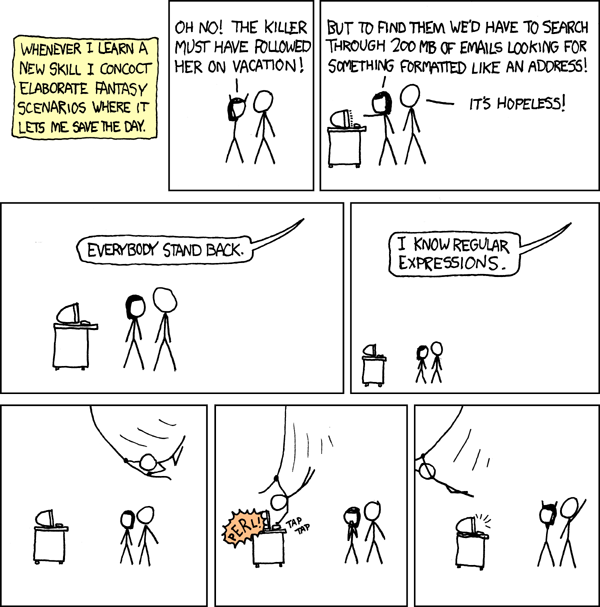
\includegraphics[scale=0.5]{xkcd_regex}

    \scriptsize Credit: \href{https://xkcd.com/208/}{https://xkcd.com/208/}
  \end{center}
\end{onlysolution}

\section*{General Remarks}
\begin{itemize}
  %
  \item If you have questions regarding the exercises, feel free to write us an email:
  \[\text{   \href{mailto:cc22@i2.informatik.rwth-aachen.de}{cc22@i2.informatik.rwth-aachen.de}}
  \]
  %
  %
  \item Exercises are \emph{optional}, i.e., not required for admission to exams. However, corrections to students’ solutions are provided as annotations to the submissions.
  %
  \item You can hand in your solution to the tasks digitaly in the Moodle room. Alternatively, you can hand in your solution to the tasks at our chair in the corresponding box or before the exercise class.
  %
  \item Please hand in your solutions in \emph{groups of four} and hand in only one solution per group. You can use the forum in this Moodle room to find group members.
\end{itemize}

\begin{exercise}{10+10+15+15}
    \begin{enumerate}
        \item Describe the language $L((01)^+(10)^+)$ in words. 
        \item Construct a regular expression over the alphabet $\Sigma=\{0,1\}$ for the set of all strings with exactly three $0$'s,
        \item Construct a regular expression over the alphabet $\Sigma=\{0,1\}$ for the set of all strings with equal number of $0$'s and $1$'s such that no prefix has two more $0$'s than $1$'s nor two more $1$'s than $0$'s.
        \item Show that there exists a language $L$ such that $L=\{0 w \ |\ w\in L\} \cup \{ 1 \}$ and $L$ is regular.
    \end{enumerate}
\end{exercise}

\begin{solution}
    \begin{enumerate}
        \item The set of all strings consisting of $0$'s and $1$'s starting and ending with $0$ and containing exactly one consecutive $1$'s but no consecutive $0$'s.
        \item The regular expression is: 
          \[1^*01^*01^*01^*\]
        \item The regular expression is:
            \[(01 | 10)^*\]
        \item Guess the solution to be  $0^*1$ (because it feels right).
            \begin{align*}
                L = \{0 w \ |\ w\in L(0^*1)\} \cup \{ 1 \}
            \end{align*}
            By substituting $L$ with $L(0^*1)$ in the equation above, we have:
            \begin{align*}
                L(0^*1) = \{0 w \ |\ w\in L(0^*1)\} \cup \{ 1 \}
            \end{align*}
            We now prove the equivalence of both sets. That is, we assume $w \in L(0^*1)$ and show that $0w$ or $1$ is in $L$ and that $w$ can be decomposed into either $1$ or $0w'$ such that $w'$ is in $L(0^*1)$.

            For the first direction we have:
            \begin{itemize}
                \item $1 \in L(0^01) \subseteq L(0^*1)$,
                \item For $w \in L(0^*1)$ we assume that $w=0^n1$. Then we have $0w = 0^{n+1}1$ and thus also $0w \in L(0^{n+1}1) \subseteq L(0^*1)$.
            \end{itemize}

            For the other direction we have: $w \in L(0^n1) \subseteq L(0^*1)$ for some $n$. We prove now that $w$ can be decomposed into either $1$ or $0w'$ such that $w' \in L(0^*1)$ by case distinction on $n$.
            \begin{itemize}
                \item For $n=0$ we have that $w=1$ and thus $w$ can be decomposed into $1$,
                \item For $n>0$ we have that $w=0^n1$ and thus $w=0w'$ with $w'=0^{n-1}1$. Remark that $w'$ is well defined because $n>0$. Finally, $w' \in L(0^{n-1}1) \subseteq L(0^*1)$.
            \end{itemize}
    \end{enumerate}
\end{solution}

%%%%%%%%%%%%%%%%%%%%%%%%%%
%
% Todo for next time:
% * what about 'It\\'s'?
% * what about 'The symbol \'?
%
%%%%%%%%%%%%%%%%%%%%%%%%%%%
\begin{exercise}{15+15+10+10}
  Let $\Omega$ be the set of all relevant characters in some encoding, e.g. all UTF-8 characters.
  In particular $\texttt{*}, \texttt{/}, \texttt{\textbackslash}, \texttt{"}, \texttt{\textquotesingle} \in \Omega$.
  \begin{enumerate}
    \item[(a)] Provide a regular expression for single-line comments (\texttt{//}) and multi-line comments (\texttt{/* ... */}) in \while (c.f.\ Programming Exercise 1).
        Please keep in mind that \texttt{*} as well as \texttt{/} may also occur inside of comments.
        Note that single-line comments are terminated by either a newline symbol \texttt{\textbackslash{}n} (Linux), a carriage return \texttt{\textbackslash{}r} (Mac OS) or both \texttt{\textbackslash{}r\textbackslash{}n} (Windows).
        Your regular expression should support comments on all three operating systems.

        \begin{minipage}{0.49\textwidth}
        Examples of \emph{valid comments} are:
        \begin{itemize}
            \item \texttt{// comment\textbackslash{}n}
            \item \texttt{/* comment \textbackslash{}r new line */}
            \item \texttt{/*foo * bar / */}
            \item \texttt{// /* test */ more comments\textbackslash{}r\textbackslash{}n}
        \end{itemize}
      \end{minipage}
      \begin{minipage}{0.49\textwidth}
        Examples of \emph{invalid comments} are:
        \begin{itemize}
            \item \texttt{// abc}
            \item \texttt{/*two*//*comments*/}
        \end{itemize}
      \end{minipage}

    \item[(b)] Provide a regular expression capturing a string.
        Strings begin and end with either double quotation marks (\texttt{"}) or single quotation marks (\texttt{\textquotesingle}).
        If a string is enclosed by double quotation marks, then single quotation marks are allowed inside the string (and vice versa).
        Lastly, an escaped quotation mark (\texttt{\textbackslash{}"} or \texttt{\textbackslash{}\textquotesingle}) is also allowed inside a string.

        \begin{minipage}{0.49\textwidth}
        Examples of \emph{valid strings} are:
        \begin{itemize}
            \item \texttt{"string"}
            \item \texttt{\textquotesingle{}02a\textbackslash{}a\textquotesingle}
            \item \texttt{"Let\textquotesingle{}s go"}
            \item \texttt{\textquotesingle{}Let\textbackslash{}\textquotesingle{}s go\textquotesingle}
        \end{itemize}
      \end{minipage}
      \begin{minipage}{0.49\textwidth}
        Examples of invalid strings are:
        \begin{itemize}
            \item \texttt{No string}
            \item \texttt{"Two""Strings"}
            \item \texttt{"String}
            \item \texttt{"He said "No""}
        \end{itemize}
      \end{minipage}

    \item[(c)] Derive \emph{one} NFA $A$ that accepts both the languages for a comment or a string as defined in the previous tasks.

    \item[(d)] Prove that $\texttt{"It\textbackslash{}\textquotesingle{}s"} \in L(A)$.
  \end{enumerate}
\end{exercise}

\begin{solution}
In the following we use the set notation $\set{a_1,\ldots,a_n}$ as a shorthand for $a_1 | a_2 | \ldots | a_n$.
\begin{enumerate}
  \item[(a)] \begin{align*}
      \mathcal{L}_{single\_cmt} ~:=~ & \texttt{//} (\Omega \setminus \set{\texttt{\textbackslash{}r}, \texttt{\textbackslash{}n}})^\ast (\texttt{\textbackslash{}n} \mid \texttt{\textbackslash{}r} \mid \texttt{\textbackslash{}r\textbackslash{}n}) \\
      %\mathcal{L}_{multi\_cmt}  ~:=~ & \texttt{/*} A^\ast (\texttt{*} B A^\ast + \texttt{*})^\ast \texttt{*/} \\
      \mathcal{L}_{multi\_cmt}  ~:=~ & \texttt{/*} \big(\texttt{/} \mid \texttt{*}^\ast (\Omega \setminus \set{\texttt{*}, \texttt{/}})\big)^\ast \texttt{*}^\ast \texttt{*/} \\
      \mathcal{L}_{comment}     ~:=~ & \mathcal{L}_{single\_cmt} \mid \mathcal{L}_{multi\_cmt}
    \end{align*}

  \item[(b)] \begin{align*}
      \mathcal{L}_{single\_string} ~:=~ & \texttt{\textquotesingle} \big( (\Omega \setminus \set{\texttt{\textquotesingle}, \texttt{\textbackslash{}}}) \mid \texttt{\textbackslash{}} \Omega \big)^\ast \texttt{\textquotesingle} \\
      \mathcal{L}_{multi\_string}  ~:=~ & \texttt{"} \big( (\Omega \setminus \set{\texttt{"}, \texttt{\textbackslash{}}}) \mid \texttt{\textbackslash{}} \Omega \big)^\ast \texttt{"} \\
      \mathcal{L}_{string}         ~:=~ & \mathcal{L}_{single\_string} \mid \mathcal{L}_{multi\_string}
    \end{align*}

  \item[(c)] We use sets as transition labels whenever there is a corresponding transition for every element of that set.

  The NFA for a comment looks as follows:
  \begin{center}
  \begin{tikzpicture}[->,>=stealth,shorten >=1pt,auto,node distance=2.5cm]
    \node[initial, initial text=,state] (N1) {$\varepsilon$};
    \node[state] (C0) [right of=N1]  {$/$};
    \node[state] (C1) [right of=C0] {$/*$};
    \node[state] (C2) [right of=C1] {$q$};
    \node[state, accepting] (C4) [right of=C2] {$cmts$};
    \node[state] (C5) [below of=C0] {$//$};
    \node[state, accepting] (C6) [right of=C5] {$p$};

  \path[->]
    (N1) edge node {/} (C0)
    (C0) edge node {*} (C1)
    (C0) edge node {/} (C5)
    (C1) edge [loop below] node {$\Omega \setminus \set{\texttt{*}}$} (C1)
    (C1) edge [bend right] node [below] {*} (C2)
    (C2) edge [bend right] node [above] {$\Omega \setminus \set{\texttt{*}, \texttt{/}}$} (C1)
    (C2) edge [loop above] node {*} (C2)
    (C2) edge node {/} (C4)
    (C5) edge [loop left] node {$\Omega \setminus \set{\texttt{\textbackslash{}n}, \texttt{\textbackslash{}r}}$} (C5)
    (C5) edge [bend right=60] node {\texttt{\textbackslash{}n}} (C4)
    (C5) edge node {\texttt{\textbackslash{}r}} (C6)
    (C6) edge node [below] {\texttt{\textbackslash{}n}} (C4)
    ;
  \end{tikzpicture}
  \end{center}

  The NFA for a string looks as follows:
  \begin{center}
  \begin{tikzpicture}[->,>=stealth,shorten >=1pt,auto,node distance=2.5cm]
    \node[initial, initial text=,state] (N1) {$\varepsilon$};
    \node[state] (S1) [above right of=N1] {\textquotesingle};
    \node[state] (M1) [below right of=N1] {"};
    \node[state] (S2) [right of=S1] {\textquotesingle\textbackslash{}};
    \node[state] (M2) [right of=M1] {"\textbackslash{}};
    \node[state, accepting] (end) [below right of=S2] {str};

  \path[->]
    (N1) edge node {\texttt{\textquotesingle}} (S1)
    (N1) edge node {\texttt{"}} (M1)
    (S1) edge[loop above] node {$\Omega \setminus \set{\texttt{\textquotesingle}, \texttt{\textbackslash}}$} (S1)
    (M1) edge[loop below] node {$\Omega \setminus \set{\texttt{"}, \texttt{\textbackslash}}$} (M1)
    (S1) edge[bend left=10] node {\texttt{\textbackslash{}}} (S2)
    (S2) edge[bend left=10] node {$\Omega$} (S1)
    (M1) edge[bend left=10] node {\texttt{\textbackslash{}}} (M2)
    (M2) edge[bend left=10] node {$\Omega$} (M1)
    (S1) edge[bend right=20] node {\texttt{\textquotesingle}} (end)
    (M1) edge[bend left=20] node {\texttt{"}} (end)
    ;
  \end{tikzpicture}
  \end{center}

  Combining both NFAs yields the NFA we are looking for:
  \begin{center}
  \scalebox{0.8}{
  \begin{tikzpicture}[->,>=stealth,shorten >=1pt,auto,node distance=2.5cm]
    \node[initial, initial text=,state] (N1) {$\varepsilon$};
    \node[state] (S1) [right of=N1] {\textquotesingle};
    \node[state] (M1) [below of=S1] {"};
    \node[state] (C1) [above of=S1] {/};
    \node (dotsC) [right of=C1] {\dots};
    \node (dotsS) [right of=S1] {\dots};
    \node (dotsM) [right of=M1] {\dots};

  \path[->]
    (N1) edge node {\texttt{/}} (C1)
    (N1) edge node {\texttt{\textquotesingle}} (S1)
    (N1) edge node {\texttt{"}} (M1)
    (S1) edge[loop above] node {$\Omega \setminus \set{\texttt{\textquotesingle}, \texttt{\textbackslash}}$} (S1)
    (M1) edge[loop below] node {$\Omega \setminus \set{\texttt{"}, \texttt{\textbackslash}}$} (M1)
    (C1) edge node {\dots} (dotsC)
    (S1) edge node {\dots} (dotsS)
    (M1) edge node {\dots} (dotsM)
    ;
  \end{tikzpicture}
  }
  \end{center}

  \item[(d)] The NFA method performs the powerset construction on the fly:
    \begin{align*}
               & (\set{\varepsilon}, \texttt{"It\textbackslash{}\textquotesingle{}s"}) \\
        \vdash & (\set{\text{"}}, \texttt{It\textbackslash{}\textquotesingle{}s"}) \\
        \vdash & (\set{\text{"}}, \texttt{t\textbackslash{}\textquotesingle{}s"}) \\
        \vdash & (\set{\text{"}}, \texttt{\textbackslash{}\textquotesingle{}s"}) \\
        \vdash & (\set{\text{"}\backslash}, \texttt{\textquotesingle{}s"}) \\
        \vdash & (\set{\text{"}}, \texttt{s"}) \\
        \vdash & (\set{\text{"}}, \texttt{"}) \\
        \vdash & (\set{\text{str}}, \varepsilon)
    \end{align*}
\end{enumerate}
\end{solution}

%\begin{exercise}{15+10+10}
\begin{enumerate}
  \item[(a)] In order to design a lexer for our Java-style programming language \while, we want to define a mapping from lexemes to symbols. Complete the following table where we already defined the lexemes and the symbol class for identifiers. Assign to each lexeme in the table an appropriate symbol class, token, and symbol. Within a symbol, the value of a lexeme can be accessed via \emph{value}. For instance, if the lexeme \emph{abc} is an identifier, then (id, \emph{abc}) is the corresponding symbol. We use the characters \textvisiblespace{} for whitespaces, \textbackslash{}t for tabular, and \textbackslash{}n and \textbackslash{}r for newlines. Other lexemes may be expressed as regular expressions or are abbreviated with $\ldots$ to increase readability.
\newcolumntype{L}{>{\ttfamily}l}
\begin{longtable}{L|l|l|l}
      \hline
      lexeme              & symbol class ~~ & token ~~~~ & symbol ~~~~ \\
      \hline
      int        &   &  &  \\
      while      &   &  &  \\
      if         &   &  &  \\
      else       &   &  &  \\

      ==         &   &  &  \\
      <          &   &  &  \\

      !          &  &  &  \\
      \&\&       &  &  &  \\
      ||         &  &  &  \\

      +          &  &  &  \\
      *          &  &  &  \\
      /          &  &  &  \\
      \%         &  &  &  \\

      ;          &  &  &  \\
      =          &  &  &  \\
      (          &  &  &  \\
      )          &  &  &  \\
      \{         &  &  &  \\
      \}         &  &  &  \\

      0 $\mid ($- $\mid \varepsilon)\{$1$,\ldots,$9$\}\{$0$,\ldots$,9$\}^\ast$ &  &  &  \\
      $\{$a,$\ldots$,z,A,$\ldots$,Z,\_$\}\{$a,$\ldots$,z,A,$\ldots$,Z,0,$\ldots$,9,\_$\}^\ast$ & identifier & id  & (id, \emph{value}) \\
      "$\{$a,$\ldots$,z,A,$\ldots$,Z,0,$\ldots$,9,\_\textvisiblespace+-*$\ldots\}^\ast$" &  &  &  \\
      true       &  &  &  \\
      false      &  &  &  \\

      //\textnormal{\ldots (}\textbackslash{}n $\mid$ \textbackslash{}r $\mid$ \textbackslash{}r\textbackslash{}n) &  &  &  \\
      /*\textnormal{\ldots}*/     &  &  &  \\
      \textvisiblespace  &  &  &  \\
      \textbackslash{}t  &  &  &  \\
      \textbackslash{}n  &  &  &  \\
      \textbackslash{}r  &  &  &  \\

      \hline
\end{longtable}



  \item[(b)] Decompose the following program (also attached as a txt file) into a sequence of lexemes and translate each lexeme into a symbol according to your solution in \textbf{(a)}.
  
  \begin{center}
  \begin{tabular}{c}
    \begin{lstlisting}
/* collatz problem */
int n = 25;
while ( 0 < n ) {
	if (n % 2 == 0) { //even?
		n =n/2;
	} else {
		n =n*3+1;
	}
}
    \end{lstlisting}
  \end{tabular}
\end{center}

 \item[(c)] Consider the following program:
 
\begin{center}
	\begin{tabular}{c}
		\begin{lstlisting}
int intx = 25;
		\end{lstlisting}
	\end{tabular}~~~~~~~~~~~~~~~~~~~~~~~~~~~~
\end{center}
%
%
Give the sequence of symbols a lexer should produce. Give two additional (but incorrect) sequences of symbols a lexer might produce. How can the lexer ensure that the decomposition of the program into lexemes is \emph{unique}?

\end{enumerate}
\end{exercise}

\begin{solution}
\newcolumntype{L}{>{\ttfamily}l} % \texttt{} version of "l" column type

\begin{enumerate}
  \item[(a)] There are several possible ways to solve this task. For example, all keywords may be identified with the same token and distinguished only through an attribute or each keyword may be identified by a unique token. The former solution is presented here, the latter is chosen for the implementation.
\begin{longtable}{Llll}
      \hline
      lexeme              & symbol class & token & symbol \\
      \hline
      int        & keywords  & key & (key, int) \\
      while      & keywords  & key & (key, while) \\
      if         & keywords  & key & (key, if) \\
      else       & keywords  & key & (key, else) \\

      ==         & relation  & rel & (rel, eq) \\
      <          & relation  & rel & (rel, lt) \\

      !          & bool. op. & bool & (bool, not) \\
      \&\&       & bool. op. & bool & (bool, and) \\
      ||         & bool. op. & bool & (bool, or) \\

      +          & arith. op. & aop & (aop, plus) \\
      *          & arith. op. & aop & (aop, mult) \\
      /          & arith. op. & aop & (aop, divide) \\
      \%          & arith. op. & aop & (aop, mod) \\

      ;          & special symbol & sym & (sym, semicolon) \\
      =          & special symbol & sym & (sym, assignment) \\
      (          & special symbol & sym & (sym, lpar) \\
      )          & special symbol & sym & (sym, rpar) \\
      \{         & special symbol & sym & (sym, lbrace) \\
      \}         & special symbol & sym & (sym, rbrace) \\

      0 $\mid ($- $\mid \varepsilon)\{$1$\ldots$9$\}\{$0$\ldots$9$\}^\ast$ & numbers & num & (num, value) \\
      $\{$a$\ldots$zA$\ldots$Z\_$\}\{$a$\ldots$zA$\ldots$Z0$\ldots$9\_$\}^\ast$ & identifier & id & (id, value) \\
      "$\{$a$\ldots$zA$\ldots$Z0$\ldots$9\_\textvisiblespace+-*$\ldots\}^\ast$" & string constant & string & (string, value) \\
      true       & boolean constant & bconst & (bconst, true) \\
      false      & boolean constant & bconst & (bconst, false) \\

      //\textnormal{\ldots (}\textbackslash{}n $\mid$ \textbackslash{}r $\mid$ \textbackslash{}r\textbackslash{}n) & comment & cmt & (cmt, cmtsingle) \\
      /*\textnormal{\ldots}*/     & comment & cmt & (cmt, cmtmulti) \\
      \textvisiblespace  & blanks & blank & none, will be ignored \\
      \textbackslash{}t  & blanks & blank & none, will be ignored \\
      \textbackslash{}n  & blanks & blank & none, will be ignored \\
      \textbackslash{}r  & blanks & blank & none, will be ignored \\

      \hline
\end{longtable}

  \item[(b)] We have the following lexemes, where we separate lexemes by a centred dot:
    \begin{itemize}
        \item[] /* collatz problem */ $\cdot$ \textbackslash{}n
        \item[] int $\cdot$ \textvisiblespace{} $\cdot$ n $\cdot$ \textvisiblespace{} $\cdot$ = $\cdot$ \textvisiblespace{} $\cdot$ 25 $\cdot$ ; $\cdot$ \textbackslash{}n
        \item[] while $\cdot$ \textvisiblespace{} $\cdot$ ( $\cdot$ \textvisiblespace{} $\cdot$ 0 $\cdot$ \textvisiblespace{} $\cdot$ < $\cdot$ \textvisiblespace{} $\cdot$ n $\cdot$ \textvisiblespace{} $\cdot$ ) $\cdot$ \textvisiblespace{} $\cdot$ \{$\cdot$ \textbackslash{}n
        \item[] \textbackslash{}t $\cdot$ if $\cdot$ \textvisiblespace{} $\cdot$ ( $\cdot$ n $\cdot$ \textvisiblespace{} $\cdot$ \% $\cdot$ \textvisiblespace{} $\cdot$ 2 $\cdot$ \textvisiblespace{} $\cdot$ == $\cdot$ \textvisiblespace{} $\cdot$ 0 $\cdot$ ) $\cdot$ \textvisiblespace{} $\cdot$ \{ $\cdot$ \textvisiblespace{} $\cdot$ //even?
        \item[] \textbackslash{}t $\cdot$ \textbackslash{}t $\cdot$ n $\cdot$ \textvisiblespace{} $\cdot$ = $\cdot$ n $\cdot$ / $\cdot$ 2 $\cdot$ ; $\cdot$ \textbackslash{}n
        \item[] \textbackslash{}t $\cdot$ \} $\cdot$ \textvisiblespace{} $\cdot$ else $\cdot$ \textvisiblespace{} $\cdot$ \{ $\cdot$ \textbackslash{}n
        \item[] \textbackslash{}t $\cdot$ \textbackslash{}t $\cdot$ n $\cdot$ \textvisiblespace{} $\cdot$ = $\cdot$ n $\cdot$ * $\cdot$ 3 $\cdot$ + $\cdot$ 1 $\cdot$ ; $\cdot$ \textbackslash{}n
        \item[] \textbackslash{}t $\cdot$ \} $\cdot$ \textbackslash{}n
        \item[] \} $\cdot$ \textbackslash{}n
    \end{itemize}

    We have the following symbol sequence (with blanks ignored):
    \begin{itemize}
        \item (cmt, cmtmulti)
        \item (key, int) (id, n) (sym, assigment) (num, 25) (sym, semicolon)
        \item (key, while) (sym, lpar) (num, 0) (rel, lt) (id, n) (sym, rpar) (sym, lbrace)
        \item (key, if) (sym, lpar) (id, n) (aop, mod) (num, 2) (rel, eq) (num, 0) (sym,rpar) (sym, lbrace) (cmt, cmtsingle)
        \item (id, n) (sym, assignment) (id, n) (aop, divide) (num, 2) (sym, semicolon)
 		\item (sym, rbrace) (key, else) (sym, lbrace)
 		\item (id, n) (sym, assignment) (id, n) (aop, mult) (num, 3) (aop, plus) (num,1) (sym, semicolon)
 		\item (sym, rbrace)
 		\item (sym,rbrace)
    \end{itemize}


\item[(c)] Correct decomposition: (key, int) (id, intx) (sym, assignment) (num,25) (sym, semicolon) \\
Incorrect decomposition (1): (key, int) (key int) (id, x) (sym, assignment)(num, 25)(sym, semicolon) \\
Incorrect decomposition (2): (id, int) (id intx) (sym, assignment)(num, 25)(sym, semicolon) \\
%
A unique decomposition of the program text into symbols can be ensured by a First-Longest-Match Analysis (cf.\ Lecture 3).
\end{enumerate}
\end{solution}





\end{document}
